\section*{}

{\centering
	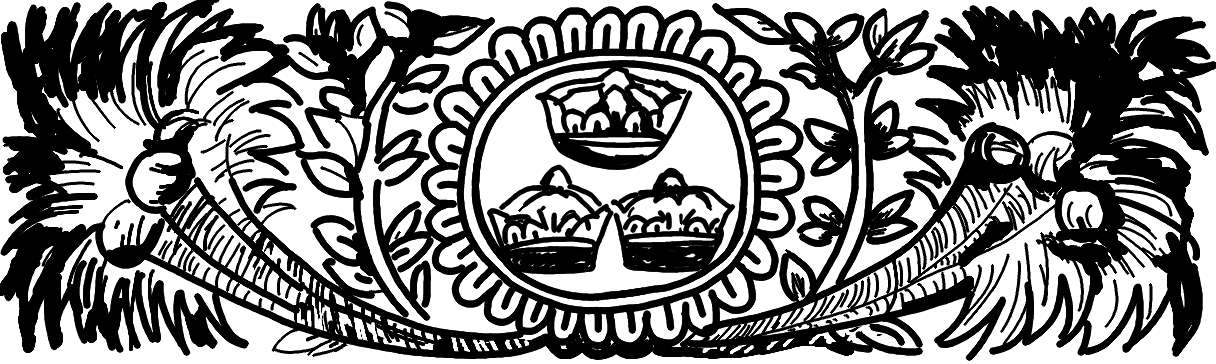
\includegraphics[scale=0.175]{images/en-tete-la-logique.png}
	\bigbreak
	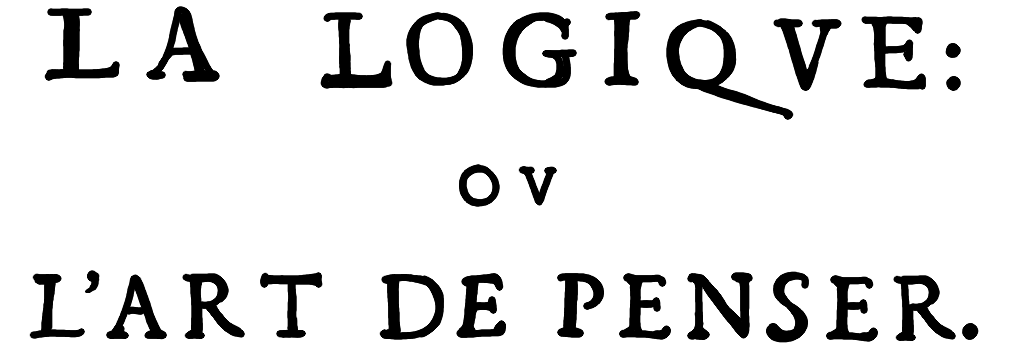
\includegraphics[scale=0.21]{images/titre-la-logique.png}
	}
\addcontentsline{toc}{section}{\scshape\large La logique ou l'art de penser}

\begin{wrapfigure}[4]{l}{0pt}
    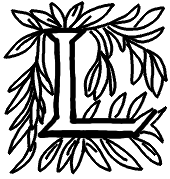
\includegraphics[width=0.20\textwidth]{images/enluminure-L0.png}
\end{wrapfigure}
\noindent\hspace{13cm}  A {A} logique est l'art de bien conduire sa raison dans la connaissance des choses, tant pour s'instruire soi-même que pour en instruire les autres.

Cet art consiste dans les réflexions que les hommes ont faites sur les quatre principales opérations de leur esprit, \emph{concevoir, juger, raisonner} et \emph{ordonner}.

On appelle \emph{concevoir}, la simple vue que nous avons des choses qui se présentent à notre esprit, comme lorsque nous nous représentons un soleil, une terre, un arbre, un rond, un carré, la pensée, l'être, sans en former aucun jugement exprès, et la forme par laquelle nous nous représentons ces choses s'appelle \emph{idée}.

On appelle \emph{juger}, l'action de notre esprit par laquelle, joignant ensemble diverses idées, il affirme de l'une qu'elle est l'autre, ou nie de l'une qu'elle soit l'autre, comme lorsqu'ayant l'idée de la Terre et l'idée du rond, j'affirme de la Terre qu'elle est ronde, ou je nie qu'elle soit ronde.

On appelle \emph{raisonner} l'action de notre esprit, par laquelle il forme un jugement de plusieurs autres ; comme lorsqu'ayant jugé que la véritable vertu doit être rapportée à Dieu, et que la vertu des païens ne lui était pas rapportée, il en conclut que la vertu des païens n'était pas une véritable vertu.

On appelle ici \emph{ordonner} l'action de l'esprit, par laquelle ayant sur un même sujet, comme sur le corps humain, diverses idées, divers jugements et divers raisonnements, il les dispose en la manière la plus propre pour faire connaître ce sujet. C'est ce qu'on appelle encore \emph{méthode}.

Tout cela se fait naturellement, et quelquefois mieux par ceux qui n'ont appris aucune règle de la logique, que par ceux qui les ont apprises.

Ainsi, cet art ne consiste pas à trouver le moyen de faire ces opérations, puisque la nature seule nous les fournit en nous donnant la raison ; mais à faire des réflexions sur ce que la nature nous fait faire, qui nous servent à trois choses.

La première est d'être assurés que nous usons bien de notre raison, parce que la considération de la règle nous y fait faire une nouvelle attention.

La seconde est de découvrir et d'expliquer plus facilement l'erreur ou le défaut qui peut se rencontrer dans les opérations de notre esprit; car il arrive souvent que l'on découvre ; par la seule lumière naturelle, qu'un raisonnement est faux, et qu'on ne découvre pas néanmoins la raison pourquoi il est faux, comme ceux qui ne savent pas la peinture peuvent être choqués du défaut d'un tableau, sans pouvoir néanmoins expliquer quel est ce défaut qui les choque.

La troisième est de nous faire mieux connaître la nature de notre esprit par les réflexions que nous faisons sur ses actions ; ce qui est plus excellent en soi, quand on n'y regarderait que la seule spéculation, que la connaissance de toutes les choses corporelles, qui sont infiniment au-dessous des spirituelles.

Que si les réflexions que nous faisons sur nos pensées n'avaient jamais regardé que nous-mêmes, il aurait suffi de les considérer en elles-mêmes, sans les revêtir d'aucunes paroles ni d'aucuns autres signes ; mais parce que nous ne pouvons faire entendre nos pensées les uns aux autres qu'en les accompagnant de signes extérieurs, et que même cette accoutumance est si forte, que quand nous pensons seuls, les choses ne se présentent à notre esprit qu'avec les mots dont nous avons accoutumé de les revêtir en parlant aux autres, il est nécessaire dans la logique de considérer les idées jointes aux mots, et les mots joints aux idées.

De tout ce que nous venons de dire, il s'ensuit que la logique peut être divisée en quatre parties, selon les diverses réflexions que l'on fait sur ces quatre opérations de l'esprit.
